\documentclass[border=8pt,tikz]{standalone}
\usepackage{tikz}
\usepackage{graphicx}
% Shared TikZ style for Chapter 5 diagrams.
% Inputted by every standalone diagram file.

\usetikzlibrary{
  arrows.meta,
  positioning,
  shapes.geometric,
  shapes.symbols,
  shapes.multipart,
  shapes.misc,
  fit,
  calc,
  backgrounds,
  decorations.pathmorphing,
  decorations.pathreplacing,
  patterns,
  shadows.blur,
}

% ─── Colour palette ──────────────────────────────────────────────
\definecolor{strixBlue}{HTML}{3B7DD8}     % data sources / inputs
\definecolor{strixGreen}{HTML}{22A699}    % processing / workers
\definecolor{strixOrange}{HTML}{E08036}   % storage
\definecolor{strixRed}{HTML}{E04B4B}      % attacker / external threat
\definecolor{strixPurple}{HTML}{6B5DD3}   % frontend / UI
\definecolor{strixGold}{HTML}{F2BE22}     % models / ML
\definecolor{strixGrey}{HTML}{6E7681}     % neutral / labels
\definecolor{strixDark}{HTML}{1F2933}     % titles / borders

% ─── Common node styles ──────────────────────────────────────────
\tikzset{
  >={Latex[width=2mm,length=2.5mm]},
  font=\sffamily\small,
  every node/.style={align=center},
  comp/.style={
    rectangle, rounded corners=2pt, draw=#1, fill=#1!10, very thick,
    text=strixDark, minimum width=22mm, minimum height=8mm,
    inner sep=4pt,
  },
  comp/.default=strixGreen,
  store/.style={
    cylinder, shape border rotate=90, aspect=0.3, draw=strixOrange,
    fill=strixOrange!12, very thick, text=strixDark,
    minimum width=18mm, minimum height=10mm, inner sep=2pt,
  },
  stream/.style={
    rectangle, rounded corners=2pt, draw=strixOrange,
    fill=strixOrange!8, dashed, thick, text=strixDark,
    minimum width=22mm, minimum height=7mm, inner sep=3pt,
    font=\ttfamily\scriptsize,
  },
  source/.style={comp=strixBlue},
  worker/.style={comp=strixGreen},
  model/.style={comp=strixGold},
  ui/.style={comp=strixPurple},
  ext/.style={comp=strixRed},
  title/.style={font=\sffamily\bfseries, text=strixDark},
  edge/.style={->, thick, draw=strixGrey, font=\sffamily\scriptsize\itshape},
  edgeStrong/.style={->, very thick, draw=strixDark, font=\sffamily\scriptsize\bfseries},
  group/.style={
    rectangle, rounded corners=4pt, draw=strixGrey, dashed, thick,
    inner sep=6pt, fill=strixGrey!4,
  },
  badge/.style={
    rectangle, rounded corners=1pt, fill=#1, text=white,
    font=\sffamily\scriptsize\bfseries, inner sep=2pt,
  },
  badge/.default=strixDark,
  port/.style={
    rectangle, rounded corners=1pt, draw=strixDark, fill=strixGrey!8,
    font=\ttfamily\scriptsize, minimum width=14mm, inner sep=2pt,
  },
}


\begin{document}
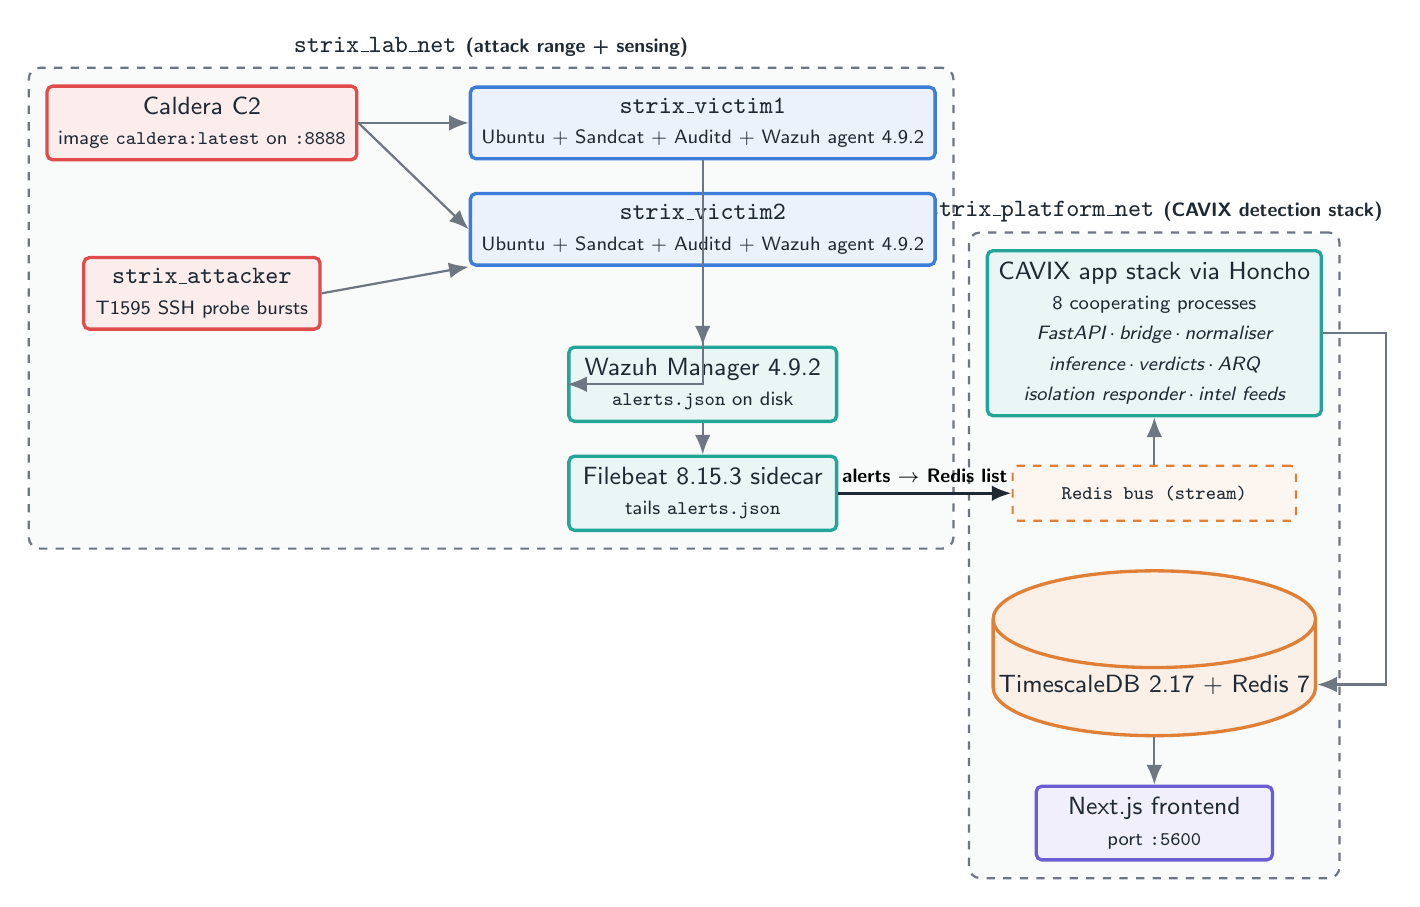
\begin{tikzpicture}[node distance=4mm and 6mm]

% ============================================================
% LEFT ZONE — strix_lab_net (attack range + sensing)
% ============================================================

\node[ext, minimum width=30mm] (caldera)
  {Caldera C2\\\scriptsize image \texttt{caldera:latest} on \texttt{:8888}};

\node[ext, minimum width=30mm, below=12mm of caldera] (attacker)
  {\texttt{strix\_attacker}\\\scriptsize T1595 SSH probe bursts};

\node[source, minimum width=42mm, right=14mm of caldera] (v1)
  {\texttt{strix\_victim1}\\\scriptsize Ubuntu + Sandcat + Auditd + Wazuh agent 4.9.2};

\node[source, minimum width=42mm, below=4mm of v1] (v2)
  {\texttt{strix\_victim2}\\\scriptsize Ubuntu + Sandcat + Auditd + Wazuh agent 4.9.2};

\node[worker, minimum width=34mm, below=10mm of v2] (wmgr)
  {Wazuh Manager 4.9.2\\\scriptsize \texttt{alerts.json} on disk};

\node[worker, minimum width=34mm, below=4mm of wmgr] (filebeat)
  {Filebeat 8.15.3 sidecar\\\scriptsize tails \texttt{alerts.json}};

% Control-plane edges (Caldera → victims, attacker → victims)
\draw[edge] (caldera.east) -- (v1.west);
\draw[edge] (caldera.east) -- (v2.west);
\draw[edge] (attacker.east) -- (v2.south west);

% Telemetry edges within the lab zone
\draw[edge] (v1.south) |- (wmgr.west);
\draw[edge] (v2.south) -- (wmgr.north);
\draw[edge] (wmgr) -- (filebeat);

% Lab group box (drawn behind the components so they remain visible)
\begin{scope}[on background layer]
  \node[group, fit=(caldera)(attacker)(v1)(v2)(wmgr)(filebeat),
        label={[font=\sffamily\bfseries\small, text=strixDark]above:%
               \texttt{strix\_lab\_net} \scriptsize (attack range + sensing)}]
        (labbox) {};
\end{scope}

% ============================================================
% RIGHT ZONE — strix_platform_net (CAVIX detection stack)
% ============================================================

\node[stream, minimum width=36mm, right=22mm of filebeat, anchor=west] (redisbus)
  {Redis bus (stream)};

\node[worker, minimum width=42mm, above=6mm of redisbus] (appstack)
  {CAVIX app stack via Honcho\\\scriptsize 8 cooperating processes\\
   \scriptsize\itshape FastAPI\,$\cdot$\,bridge\,$\cdot$\,normaliser\\
   \scriptsize\itshape inference\,$\cdot$\,verdicts\,$\cdot$\,ARQ\\
   \scriptsize\itshape isolation responder\,$\cdot$\,intel feeds};

\node[store, minimum width=36mm, below=6mm of redisbus] (db)
  {TimescaleDB 2.17 + Redis 7};

\node[ui, minimum width=30mm, below=6mm of db] (web)
  {Next.js frontend\\\scriptsize port \texttt{:5600}};

% Edges within platform
\draw[edge] (redisbus) -- (appstack);
\draw[edge] (appstack.east) -- ++(8mm,0) |- (db.east);
\draw[edge] (db.south) -- (web.north);

% Platform group box (background layer so contents stay visible)
\begin{scope}[on background layer]
  \node[group, fit=(redisbus)(appstack)(db)(web),
        label={[font=\sffamily\bfseries\small, text=strixDark]above:%
               \texttt{strix\_platform\_net} \scriptsize (CAVIX detection stack)}]
        (platbox) {};
\end{scope}

% ============================================================
% Cross-boundary arrow (the only data path between the two zones)
% ============================================================
\draw[edgeStrong] (filebeat.east) --
  node[above, font=\sffamily\scriptsize\bfseries] {alerts $\rightarrow$ Redis list}
  (redisbus.west);

\end{tikzpicture}
\end{document}
